%定义文档类型和基本的页面设置
\documentclass[12pt,a4paper]{article}

%加载要用到的宏包
\usepackage[utf8]{inputenc}
\usepackage{amsmath}
\usepackage{amsfonts}
\usepackage{amssymb}
\usepackage{amsthm}
\usepackage{bussproofs}
\usepackage{tikz}
\usepackage[left=1.5cm,right=1.5cm]{geometry}

%自定义环境
\theoremstyle{plain}
\newtheorem{exercise}{Exercise}

%文档的标题
\title{Homework 5}

%文档的作者
\author{(WEI Lai)\\
(1801211383)}

%文档的日期
\date{Deadline: 23:59, November 8th, 2018}

%文档内容开始
\begin{document}

%打出文档的标题、作者、日期等信息
\maketitle

Please do Exercises 3.3.10 (b), 3.4.6(b) and 3.4.6 (d) in the textbook and compare your solutions to those at the end of the book.

You do NOT need to hand in your solutions to the above exercises.

\ \\
\begin{exercise}
Please solve Exercise 3.3.6 in the textbook:

\ \\
Item (a) below gives us a second method for showing that a given expression is not a formula of LP($\sigma$) for a given signature $\sigma$.
Its advantage is that you normally do not need parsing trees for it. 
Its disadvantage is that you have to have an idea, unlike the method of Example 3.3.6 which is an algorithm that could be done by a computer.
%
\begin{itemize}

\item[(a)] Prove the following: let $S$ be a set of expressions such that 
%
\begin{itemize}

\item[(1)] every atomic formula of LP($\sigma$) is in $S$;

\item[(2)] if $s$ and $t$ are any expressions in $S$, then the expressions
%
\[
(\neg s) \quad (s \wedge t) \quad (s \vee t) \quad (s \rightarrow t) \quad (s \leftrightarrow t)
\]
%
are all in $S$.

\end{itemize} 
%
Then every formula of LP($\sigma$) is in $S$.

[Let $\pi$ be a parsing tree. 
Show (by induction on height of $\nu$) that if (1) and (2) are true then for every node $\nu$ of $\pi$, the formula $F_\pi (\nu)$ at $\nu$ is in $S$.]

\item[(b)] Use (a) to show that every formula of LP($\sigma$) has equal numbers of left parentheses `(' and right parentheses `)'. 
[Put $S = \{s \mid s$ has equal numbers of left and right parentheses$\}$, and remember to prove that (1) and (2) are true for this $S$.] 

Deduce that
%
\[
(((p \rightarrow q) \vee (\neg p))
\]
%
is not a formula of LP($\sigma$).

\end{itemize}
\end{exercise}

\begin{proof}
(Please write your proof here.)
\end{proof}

\ \\
\begin{exercise}
Please solve Exercise 3.3.8 (c) and (d) in the textbook:

\ \\
The Unique Parsing Theorem makes essential use of the parentheses `(' and `)' in a formula. 
But there are other logical notations that do not need parentheses. 
For example, \emph{Polish} (also known as \emph{head-initial}) notation has the following compositional definition:
%
\begin{center}
\begin{tabular}{ccc}
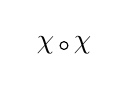
\begin{tikzpicture}
[level distance=1.5cm]
\tikzstyle{hollow node}=[circle,draw,inner sep=1]

\node(0)[hollow node]{};
   
\node[left]at(0){$\chi$};
\node[right]at(0){$\chi$};
\end{tikzpicture}
\qquad & \qquad
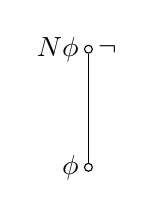
\begin{tikzpicture}
[level distance=1.5cm]
\tikzstyle{hollow node}=[circle,draw,inner sep=1]

\node(0)[hollow node]{} 
[sibling distance=25mm]
   child{node(1)[hollow node]{}};
   
\node[left]at(0){$N\phi$};
\node[right]at(0){$\neg$};
\node[left]at(1){$\phi$};
\end{tikzpicture}
\qquad & \qquad
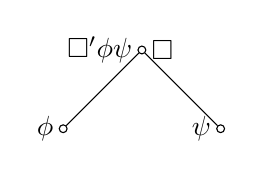
\begin{tikzpicture}
[level distance=1cm]
\tikzstyle{hollow node}=[circle,draw,inner sep=1]

\node(0)[hollow node]{} 
[sibling distance=20mm]
     child{node(1)[hollow node]{}}
     child{node(2)[hollow node]{}};
   
\node[left]at(0){$\Box' \phi \psi$};
\node[right]at(0){$\Box$};
\node[left]at(1){$\phi$};
\node[left]at(2){$\psi$};
\end{tikzpicture}
\end{tabular}
\end{center}
%
where $\chi$ is atomic, $\Box \in \{ {\wedge} , {\vee} , {\rightarrow} , {\leftrightarrow} \}$, ${\wedge}'$ is $K$, ${\vee}'$ is $A$, ${\rightarrow}'$ is $C$ and ${\leftrightarrow}'$ is $E$.
%
\begin{itemize}

\item[(c)] Translate the following formulas from LP notation to Polish notation:
%
\begin{itemize}

\item[(i)] $(p \wedge (q \vee (\neg p)))$.

\item[(ii)] $(((p \rightarrow q) \rightarrow p) \rightarrow p)$.

\end{itemize}

\item[(d)] Translate the following formulas from Polish notation to LP notation:
\begin{itemize}

\item[(i)] $EApqNKNpNq$.

\item[(ii)] $CCqrCCpqCpr$.

\end{itemize}

\end{itemize}
\end{exercise}

\begin{proof}[Solution]
(Please write your solution here.)
\end{proof}

\ \\
\begin{exercise}
Please solve Exercise 3.4.1 in the textbook: (You are free to follow either the style in the textbook or the style in the slides.
You do NOT need to draw diagrams similar to those in the slides.)

\ \\
Add the missing clauses (d)(iii)–(v) and (e)(ii)–(iv) to Definition 3.4.1.
\end{exercise}

\begin{proof}[Solution]
(Please write your solution here.)
\end{proof}

\ \\
\begin{exercise}
Please solve Exercise 3.4.2 (b) in the textbook:

\ \\
Let $\sigma$ be the default signature $\{ p_0 , p_1 , \dots \}$. 
Neither of the following two diagrams is a $\sigma$-derivation.
 In them, find all the faults that you can, and state which clause of Definition 3.4.1 is violated by each fault. 
(Consider the diagrams as shorthand for labelled trees, as (3.33) is shorthand for (3.34).)

\begin{prooftree}
\AxiomC{$[ ( \neg ((\neg p_2) \vee q )) ]$($\alpha$)}
\AxiomC{$[ ( \neg p_2 ) ]$($\beta$)}
\RightLabel{($\vee$I)($\gamma$)}
\UnaryInfC{$((\neg p_2) \vee q )$}
\RightLabel{($\neg$E)($\delta$)}
\BinaryInfC{$\bot$}
\RightLabel{($\neg$I)($\epsilon$)}
\UnaryInfC{$p_2$}
\AxiomC{$[ p_2 ]$($\zeta$)}
\AxiomC{$[ p_2 \rightarrow q ]$($\eta$)}
\RightLabel{($\rightarrow$E)($\theta$)}
\BinaryInfC{$q$}
\RightLabel{($\vee$I)($\iota$)}
\UnaryInfC{$( ( \neg p_2 ) \vee q )$}
\AxiomC{$[ ( \neg ( ( \neg p_2 ) \vee q ) ) ]$($\kappa$)}
\RightLabel{($\lambda$)}
\BinaryInfC{$\bot$}
\RightLabel{(RAA)($\mu$)}
\UnaryInfC{$( \neg p_2 )$}
\RightLabel{($\neg$I)($\nu$)}
\BinaryInfC{$\bot$}
\RightLabel{($\neg$I)($\xi$)}
\UnaryInfC{$( ( \neg p_2 ) \vee q )$}
\end{prooftree}
\end{exercise}

\begin{proof}[Solution]

($\delta$) violates Clause (e)(iii), for the left labels on the daughters of the node with right label ($\neg$E) are not (from left to right) $((\neg p_2) \vee q )$ and $( \neg ((\neg p_2) \vee q ))$.

(Please continue by writing your answer here.)
\end{proof}

\ \\
\begin{exercise}
Please solve Exercise 3.4.6 (a) and (c) in the textbook: (You may study as examples the solutions to (b) and (d) at the end of the book.)

\ \\
We have stated several rules about correct sequents, and verified them informally. 
With our new formal definition of sequents we can prove them mathematically.
Do so using Definition 3.4.1. 
(The formulas mentioned are all assumed to be in LP($\sigma$).)
%
\begin{itemize}

\item[(a)] The Axiom Rule: If $\psi$ is a formula in $\Gamma$ then $( \Gamma \vdash_\sigma \psi )$ is correct.

\item[(c)] The Transitive Rule: If $(\Delta \vdash_\sigma \psi)$ is correct and for every formula $\chi$ in $\Delta$, $(\Gamma \vdash_\sigma \chi )$ is correct, then $(\Gamma \vdash_\sigma \psi)$ is correct.

\end{itemize}
\end{exercise}

\begin{proof}
(Please write your proof here.)
\end{proof}

%文档内容结束
\end{document}